\newcommand{\todo}[1]{{\bf TODO} #1}
\newif\ifPAPER  
%\PAPERtrue % select either slide or note
\PAPERfalse  

\def\t{\title{Simulating carbon beam fragmentation on water phantom with the Geant4 INCL/ABLA models}}

\def\a{
\author{A.~Heikkinen} 
\affiliation{Helsinki Institute of Physics, P.O. Box 64, FIN-00014 University of Helsinki (Finland)}
}

\newcommand{\codeAlgorithm}[1]{
\addcontentsline{toc}{section}{Résumé}
\begin{center}\fbox{\parbox{12cm}{\bf #1}}\end{center}}

\newcommand{\cppintro}[1]{
\lstset{language=C,
caption= #1 ,
label=listing:boundary}}

\def\cppstart{\begin{lstlisting}}
\def\cppend{\end{lstlisting}}

\newif\ifCITENOTE 
\CITENOTEtrue

\ifPAPER

\else   % Slides ---------------------------------------------------------------

\documentclass[slidestop,compress,xdvips,10pt]{beamer} 
\usetheme{Antibes}
\usecolortheme{lily}
\usepackage{graphicx}
\usepackage{hyperref}
\usepackage{listings}
\usepackage{verbatim} % for comment
\transglitter[direction=315]
\xdefinecolor{ahcol}{rgb}{0.2, 0.4, 0.1}
\xdefinecolor{olive}{cmyk}{0.64,0,0.95,0.4}
\colorlet{structure}{green!60!black} % for color substitution
\usepackage{color} % for definecolor
\definecolor{light-gray}{gray}{0.95}
\definecolor{dark-gray}{gray}{0.30}
\definecolor{orange}{rgb}{1,0.5,0}
\definecolor{dark-blue}{cmyk}{1,0.5,0.5,0}
\usepackage{attachfile} 
\hypersetup{
    a4paper, % page format
    pdftitle={My Title},                  % Title
    pdfsubject={Subject of the document}, % Subject 
    pdfauthor={Author name},              % Author
    pdfkeywords={list of keywords},       % Keywords
    plainpages=true, %
    colorlinks,       % links are colored
    urlcolor=dark-blue,    % color of external links
    linkcolor=dark-blue,    % color of internal links
    citecolor=black,  % color of links to bibliography
    bookmarksnumbered
}

\usecolortheme[named=ahcol]{structure}
\useoutertheme{myinfolines}
\useinnertheme{rounded}
\setbeamercolor{alerted_text}{fg=blue}

\makeatother
\beamertemplatetransparentcoveredhigh
\t
\author{\underline{A.~Heikkinen}
\footnote{Helsinki Institute of Physics, P.O. Box 64, FIN-00014 University of Helsinki, Finland.
aatos.heikkinen@cern.ch}}

%\author{Aatos Heikkinen 
%\footnote{Helsinki Institute of Physics, Helsinki, Finland.
%%{\tt aatos.heikkinen@cern.ch}} and Ivica Puljak 
%\footnote{University of Split - FESB, Split, Croatia}
%}
\graphicspath{{.}{figures/}}
\graphicspath{{images/}}
\begin{document}

%\begin{comment}
\frame{\titlepage}
%\end{comment}

\section{}

\subsection{}
\frame{
\frametitle{Outline}
\begin{itemize}
\item INCL cascade and ABLA evaporation/fission models in Geant4 9.2.

\item New Geant4 physics list for spallation studies.
\item Examples of INCL/ABLA physics performance.

\item Validation of Geant4 against data from GSI $^{12}$C beam fragmentation in water target:
\begin{itemize}
\item Our plan is that this study will evolve as Geant4 benchmarking platform for
the Coordinated Research Project (CRP) on
\href{http://www-nds.iaea.org/charpar/charpar.htmlx}{Heavy Charged-Particle Interaction 
Data for Radiotherapy}.
\end{itemize}
\end{itemize}
\vspace{0.3cm}
This work is done in collaboration with
Alain Boudard\footnote{CEN-Saclay, CEA-IRFU/SPhN, 91 191 Gif sur Yvette, France},
Pekka Kaitaniemi\footnote{CEN-Saclay and Helsinki Institue of Physics}, 
and Gillis Danielsen\footnote{Helsinki University of Technology}.

\vspace{0.3cm}
Plans to extend Hadrontherapy example to implement the CRP in Geant4 are made in collaboration with
its main developers (G.A.P. Cirrone, G.Cuttone, F.Romano, {\em et al.}) 
and J.~M.~Quesada (Universidad de Sevilla).

}

\frame{
\frametitle{INCL: $^{12}$C 500~MeV/A + Fe \footnote{From \cite{boudard09a}}}
\vspace{0.1cm}
\begin{center}
%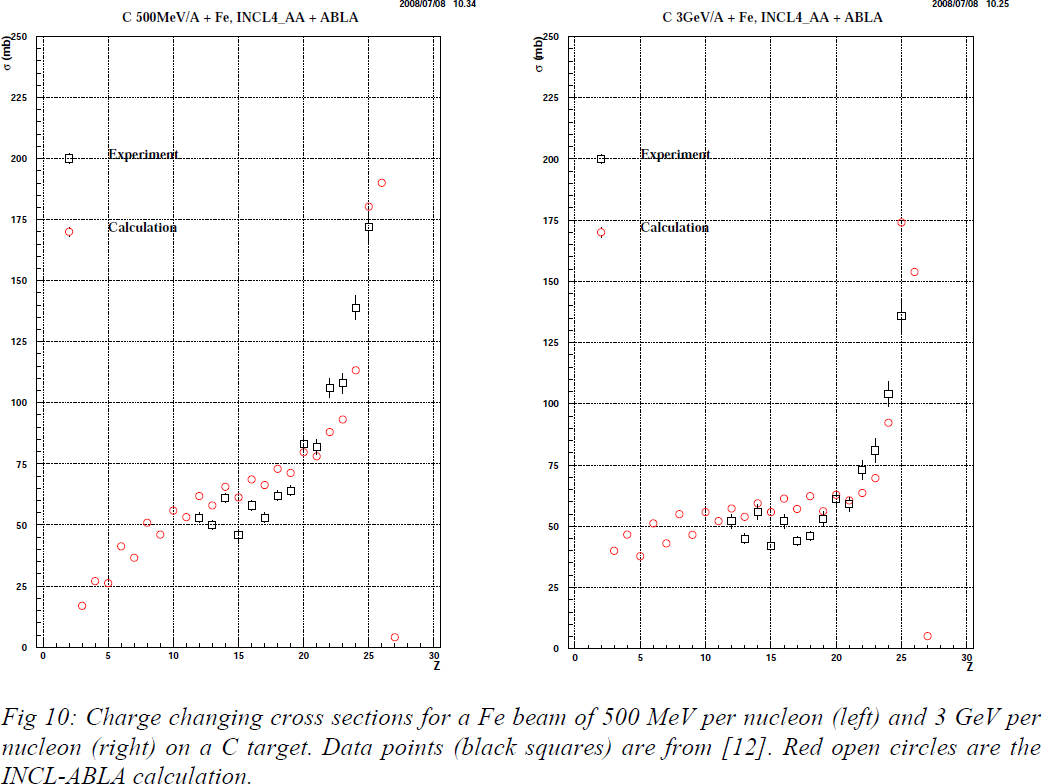
\includegraphics[width=0.75\textwidth]{chargeChanging}
\end{center}
}


\begin{frame}[allowframebreaks]{References}
\bibliographystyle{alpha}  % Options plain, unsrt, alpha, abbrv
\bibliography{refs} %10 p
\end{frame}
\end{document}

\fi %slides



